\section{Data Unification}
\label{sec:unification}
In this section we point out the data streams' characteristics obtainable from our two sample open data clouds and how we aim to unify them onto a single data cloud.
We extracted the whole repositories and parsed the JSON files in order to give a first structure to such data.
Since the data structure does not force strong constraints data is often incomplete in such a way that, in some cases, it is not usable.
This happens when no location information is given, the stream name and the description is not understandable, the stream has not been recently updated and so on.
\\

\begin{figure*}[t]
\centering
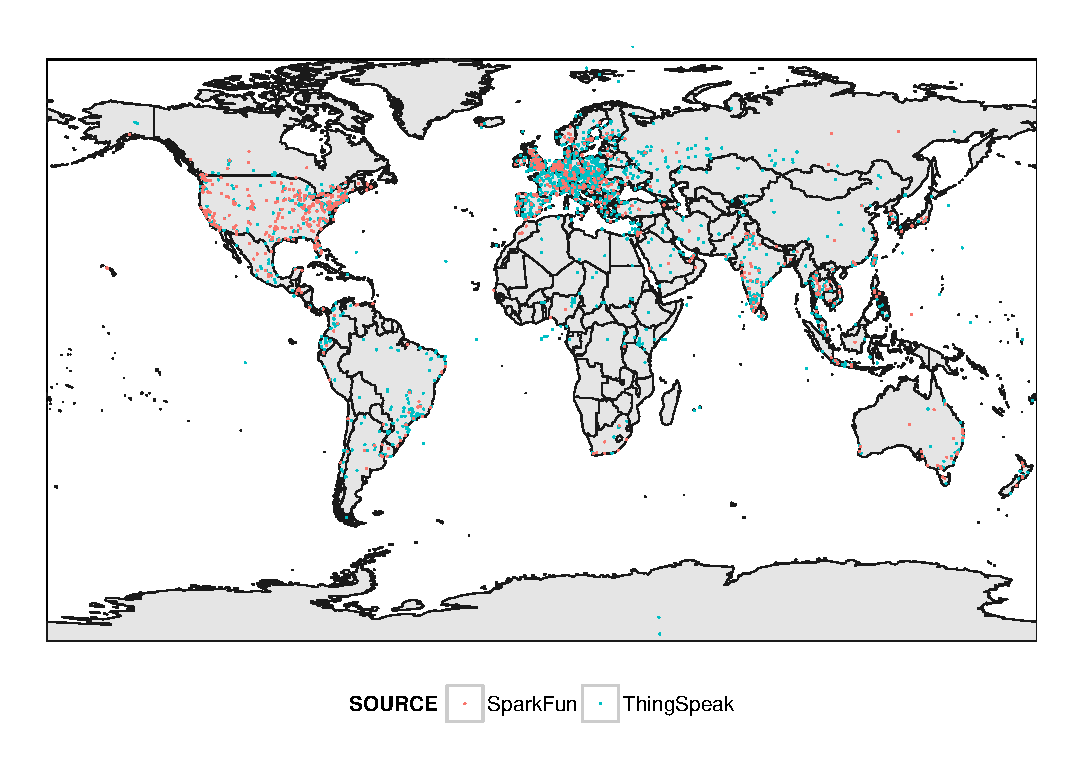
\includegraphics[width=0.96\textwidth]{img/map.eps} 
\caption{Location of all ThingSpeak and SparkFun sensing sources.}
\label{geo}
\end{figure*}

Hereby are briefly presented some of the metadata that can be extracted from data streams:
\begin{itemize}
 \item \textbf{Stream ID}: it is the data stream's unique ID. In ThingSpeak it is represented by an incremental number, which is assigned when the stream is created. At the time of writing there are 28806 active and public streams with IDs spanning from 0 to 100172. In SparkFun the unique ID is given by a string of 20 random ASCII characters. At the time of writing we counted 3575 different SparkFun streams. 
 \item \textbf{Stream name}: it present in both platforms and it is determined by the user with no constraint. It might carry or not useful information about the stream.
 \item \textbf{Geolocalization}: it is present in both platforms. In ThingSpeak not all the streams come with GPS data. Similarly, in SparkFun not all the streams are geolocalized, however, when they are, only the name of the city, or sometimes just the state or even just the country, is given. When extracting data in JSON from SparkFun, GPS coordinates are given, however we observed that such coordinates are probably obtained through some API converting the name of the city, since streams coming from the same city have the same GPS coordinates.
 \item \textbf{Tags}: are included in both platforms and represent the keywords that users assign to streams. They often help to infer useful information about the data. 
 \item \textbf{Creation Timestamp}: it is included in all ThingSpeak and SparkFun streams as a metadata. It usually does not correspond to the timestamp relative to the first registered update, since each stream has a limited number of updates staying registered, then the platform erases the first updates in excess. In SparkFun the limit is 50 MB, while in ThingSpeak is 100 updates.
 \item \textbf{Last Update Timestamp}: it is included in all ThingSpeak streams as a metadata. In SparkFun is simply deducible from the timestamp of the last update in the stream, since the timestamp is implicitly included for each update.
 \item \textbf{Description}: it is a ThingSpeak metadata and its characterization is fully assigned to the user (who can also decide not to include it).
 \item \textbf{Elevation}: it is a ThingSpeak metadata and not always indicated, it represents the location of the stream's source on the $z$ axis, i.e. its vertical distance in meters from the sea level.
 \item \textbf{Metadata}: it is a non-mandatory ThingSpeak metadata which contains additional data for the stream in plain text. It is suitable for structured data such JSON and XML.
 \item \textbf{Url}: it is a non-mandatory ThingSpeak metadata indicating the address of the official web page of the stream.
 \item \textbf{Last Entry ID}: it is a ThingSpeak metadata, which points to the last update record in the data, ordered using an incremental ID for each update.
\end{itemize}

Each data stream can contain different data fields.
An example is given by the streams making use of the popular DHT11 or DHT22 sensors, which are devoted to sense temperature and humidity and, therefore, such channels have two fields.
Data fields, both in ThingSpeak and SparkFun, also have names, which represent the only way to discriminate which field registers which measurement.
In both platforms each measurement comes together with an integrated timestamp.

From each data stream we extracted in particular the GPS position for a location analysis, finding that such position is indicated, with different degree of precision, in 6665 data streams out of 32381 (nearly 21\%). Thingspeak accounts for a total of nearly 14\% of geolocalized data streams, while Sparkfun takes the remaining 7\%. However as stated before, the GPS position provided by SparFun indicates the center of the entity (the city, or the region) where the source is located.
The results of the analysis are outlined in Figure~\ref{geo}.

Given such results, the importance of information fusion from different sources is clear, since merging such sources not only increments the sampling number of the sensing infrastructure, but also its coverage.
Indeed, ThingSpeak appears to have much more utilization in the European region, whereas SparkFun seems to be more popular in North America.
Furthermore, this consideration might be extended to different macro topic areas, meaning that some open data sources are specialized on a specific field of measuring.
For instance, governmental sources providing open data such as EPA (United States Environmental Protection Agency) \cite{epa} are primarily focused on environmental data, whilst crowdsensing sources such as OpenSignal \cite{opensignal} regard measurements on cellular network signal strength and coverage.

\begin{figure*}[!t]
\centering
\includegraphics[width=0.96\textwidth]{img/Archit.eps} 
\caption{Our proposed architecture.}
\label{arch}
\end{figure*}

Therefore, a basic unification counting on an essential set of metadata is crucial, composing the minimum skeleton to which a data stream should be linked.
For such purpose we aim to design an unique ID assignment policy, a geolocalization (in GPS coordinates with a precision error), the freshness of the information (given by the last update timestamp), when it was created (given by the stream creation date), a friendly name and an inferred measurement category for each field (such as temperature, humidity and so on) together with an unit of measure.
The latter is essential, since most applications need to use services providing a certain type of information, which will be given by the class assigned to the measurement field.
Without such a semantic approach, each data stream will have no meaning.

